% Options for packages loaded elsewhere
\PassOptionsToPackage{unicode}{hyperref}
\PassOptionsToPackage{hyphens}{url}
\PassOptionsToPackage{dvipsnames,svgnames,x11names}{xcolor}
%
\documentclass[
  authoryear,
  preprint,
  3p]{elsarticle}

\usepackage{amsmath,amssymb}
\usepackage{iftex}
\ifPDFTeX
  \usepackage[T1]{fontenc}
  \usepackage[utf8]{inputenc}
  \usepackage{textcomp} % provide euro and other symbols
\else % if luatex or xetex
  \usepackage{unicode-math}
  \defaultfontfeatures{Scale=MatchLowercase}
  \defaultfontfeatures[\rmfamily]{Ligatures=TeX,Scale=1}
\fi
\usepackage{lmodern}
\ifPDFTeX\else  
    % xetex/luatex font selection
\fi
% Use upquote if available, for straight quotes in verbatim environments
\IfFileExists{upquote.sty}{\usepackage{upquote}}{}
\IfFileExists{microtype.sty}{% use microtype if available
  \usepackage[]{microtype}
  \UseMicrotypeSet[protrusion]{basicmath} % disable protrusion for tt fonts
}{}
\makeatletter
\@ifundefined{KOMAClassName}{% if non-KOMA class
  \IfFileExists{parskip.sty}{%
    \usepackage{parskip}
  }{% else
    \setlength{\parindent}{0pt}
    \setlength{\parskip}{6pt plus 2pt minus 1pt}}
}{% if KOMA class
  \KOMAoptions{parskip=half}}
\makeatother
\usepackage{xcolor}
\setlength{\emergencystretch}{3em} % prevent overfull lines
\setcounter{secnumdepth}{5}
% Make \paragraph and \subparagraph free-standing
\ifx\paragraph\undefined\else
  \let\oldparagraph\paragraph
  \renewcommand{\paragraph}[1]{\oldparagraph{#1}\mbox{}}
\fi
\ifx\subparagraph\undefined\else
  \let\oldsubparagraph\subparagraph
  \renewcommand{\subparagraph}[1]{\oldsubparagraph{#1}\mbox{}}
\fi


\providecommand{\tightlist}{%
  \setlength{\itemsep}{0pt}\setlength{\parskip}{0pt}}\usepackage{longtable,booktabs,array}
\usepackage{calc} % for calculating minipage widths
% Correct order of tables after \paragraph or \subparagraph
\usepackage{etoolbox}
\makeatletter
\patchcmd\longtable{\par}{\if@noskipsec\mbox{}\fi\par}{}{}
\makeatother
% Allow footnotes in longtable head/foot
\IfFileExists{footnotehyper.sty}{\usepackage{footnotehyper}}{\usepackage{footnote}}
\makesavenoteenv{longtable}
\usepackage{graphicx}
\makeatletter
\def\maxwidth{\ifdim\Gin@nat@width>\linewidth\linewidth\else\Gin@nat@width\fi}
\def\maxheight{\ifdim\Gin@nat@height>\textheight\textheight\else\Gin@nat@height\fi}
\makeatother
% Scale images if necessary, so that they will not overflow the page
% margins by default, and it is still possible to overwrite the defaults
% using explicit options in \includegraphics[width, height, ...]{}
\setkeys{Gin}{width=\maxwidth,height=\maxheight,keepaspectratio}
% Set default figure placement to htbp
\makeatletter
\def\fps@figure{htbp}
\makeatother

\usepackage{booktabs}
\usepackage{longtable}
\usepackage{array}
\usepackage{multirow}
\usepackage{wrapfig}
\usepackage{float}
\usepackage{colortbl}
\usepackage{pdflscape}
\usepackage{tabu}
\usepackage{threeparttable}
\usepackage{threeparttablex}
\usepackage[normalem]{ulem}
\usepackage{makecell}
\usepackage{xcolor}
\makeatletter
\@ifpackageloaded{caption}{}{\usepackage{caption}}
\AtBeginDocument{%
\ifdefined\contentsname
  \renewcommand*\contentsname{Table of contents}
\else
  \newcommand\contentsname{Table of contents}
\fi
\ifdefined\listfigurename
  \renewcommand*\listfigurename{List of Figures}
\else
  \newcommand\listfigurename{List of Figures}
\fi
\ifdefined\listtablename
  \renewcommand*\listtablename{List of Tables}
\else
  \newcommand\listtablename{List of Tables}
\fi
\ifdefined\figurename
  \renewcommand*\figurename{Figure}
\else
  \newcommand\figurename{Figure}
\fi
\ifdefined\tablename
  \renewcommand*\tablename{Table}
\else
  \newcommand\tablename{Table}
\fi
}
\@ifpackageloaded{float}{}{\usepackage{float}}
\floatstyle{ruled}
\@ifundefined{c@chapter}{\newfloat{codelisting}{h}{lop}}{\newfloat{codelisting}{h}{lop}[chapter]}
\floatname{codelisting}{Listing}
\newcommand*\listoflistings{\listof{codelisting}{List of Listings}}
\makeatother
\makeatletter
\makeatother
\makeatletter
\@ifpackageloaded{caption}{}{\usepackage{caption}}
\@ifpackageloaded{subcaption}{}{\usepackage{subcaption}}
\makeatother
\journal{Journal Name}
\ifLuaTeX
  \usepackage{selnolig}  % disable illegal ligatures
\fi
\usepackage[]{natbib}
\bibliographystyle{elsarticle-harv}
\usepackage{bookmark}

\IfFileExists{xurl.sty}{\usepackage{xurl}}{} % add URL line breaks if available
\urlstyle{same} % disable monospaced font for URLs
\hypersetup{
  pdftitle={A multi-scale story of the diffusion of a new technology: the web},
  pdfauthor={Emmanouil Tranos},
  pdfkeywords={keyword1, keyword2},
  colorlinks=true,
  linkcolor={blue},
  filecolor={Maroon},
  citecolor={Blue},
  urlcolor={Blue},
  pdfcreator={LaTeX via pandoc}}

\setlength{\parindent}{6pt}
\begin{document}

\begin{frontmatter}
\title{A multi-scale story of the diffusion of a new technology: the
web}
\author[1]{Emmanouil Tranos%
\corref{cor1}%
}
 \ead{e.tranos@bristol.ac.uk} 

\affiliation[1]{organization={University of Bristol and The Alan Turing
Institute},postcode={UK},postcodesep={}}

\cortext[cor1]{Corresponding author}

        
\begin{abstract}
This paper maps the participation in the digital economy and its
evolution in the UK over space and time. Most of the existing economic
geography literature which dealt with the spatiality of the internet
employed supply-side measures, such as infrastructural capacity, in
order to understand the geography of the digital economy and its
potential spatial economic effects. Useful as these approaches might
have been, they cannot capture the micro-processes and the
characteristics of the individual online behaviour. Using large volumes
of archived and geolocated web content, this paper models the diffusion
of web technologies over space and time in the UK. The data and
geolocation strategy allow to capture these processes at a very granular
spatial scale. The modelling approach, which is based on simple spatial
analytical methods and on the estimation of diffusion curves at various
scales, enables to depict the role of geography and other cognitive
factors which drove the diffusion of web technologies. Although the
focus is on a recent historical period -- 1996-2012 -- the results of
the analysis depict diffusion mechanisms which can be very useful in
understanding the evolutionary patterns of the adoption of other newer
technologies.
\end{abstract}





\begin{keyword}
    keyword1 \sep 
    keyword2
\end{keyword}
\end{frontmatter}
    
\section{Introduction}\label{sec1}

Geographers were always interested in how new technologies and
innovations diffuse across space and time and, importantly, how such
spatio-temporal processes can be modeled. After all, diffusion together
with invention and innovation are considered the pillars of
technological change \citep{das2022diffusion}. The seminal contribution
of \citet{hagerstrand1968innovation} is illustrative of this early
interest. However, the torch of exploring and modelling such processes
had been passed to other disciplines such as economics, business studies
and sociology well before the `cultural turn' of economic geography
\citep{perkins2005international}. A potential explanation of the lack of
geographical studies exploring the diffusion of new and, more
specifically for this paper, digital technologies across both space and
time can be attributed to the scarcity of relevant and granular enough
data. As \citet{zook2022mapping} highlight, digital activities are
hardly ever captured in official data.

This paper offers such a contribution: a geographical study illustrating
how a new technology that is the web diffused over space and time in the
UK at a high level of spatial granularity during the \(1996-2012\)
period. It does so by employing a novel source of big data which
captures the active engagement with web technologies during that period.
By addressing this empirical question this paper exemplifies how the
combination of data sources which escape the traditional social science
domain and adequate research methods can offer new lenses to
geographical research regarding the understanding of technological
diffusion.

\textbf{SAY SOMETHING ABOUT SPATIAL ANALYTICS, DIST PAPER BY ARP, NOT
SPECIFIC EXPLANATORY VARIABLES, INTANGIBLE}

The motivation for this paper lies in the fact that there are various
stakeholders who are interested in knowing how new digital technologies
diffused over space and time and use this knowledge to make predictions
regarding the diffusion of related \emph{future} technologies. As per
\citet{leibowicz2016representing}, historical studies agree on the fact
that ``technologies diffuse at different times, at different rates, and
to different extents in different places, and can be significantly
influenced by policies'' \citep{victor1993}. \citet{meade2021modelling}
highlight that a variety of actors have a direct interest in gaining
such knowledge including network equipment suppliers; network operators,
regulatory and local authorities. These processes and their effects vary
a lot across scales: although the diffusion of a new technology might
not be optimal at a local level, it might be beneficial from a global
perspective as it could lead to faster diffusion to less advantaged
places \citep{leibowicz2016representing}. Despite the spatial
heterogeneity of such diffusion mechanisms and the policy relevance,
there are very limited attempts in the literature to analyse the
diffusion of new digital technologies at a detailed geographical level.

Technological diffusion, which is by definition an aggregated process,
can be discussed in parallel with individual adoption mechanisms. On the
one hand, \citet{rogers2010diffusion} identifies early adopter of new
technologies as `knowledgeable risk takers' and \citet{griliches1957} as
`profit maximisers' \citep{ding2010modeling}. Such individual agents are
rewarded because of their attitude towards new technologies and
innovations. On the other hand, \citet{perkins2011internet} attribute
diffusion to two processes: (i) epidemic-like mechanisms, which are
governed by distance, proximity and social interactions, and (ii) by
economic mechanisms as new innovations are adopted by users as they
become more profitable, valueable and useful.

This paper focuses on the diffusion of the web as new technology during
the \(1996-2012\) period. This was an exciting period for digital
technologies as it corresponds with the commercialisation of the
internet and, consequently, its almost universal adoption. The reader is
reminded that it was only in 1994 when Netscape Navigator was
introduced, a year before Microsoft's Internet Explorer.\footnote{\url{https://www.theguardian.com/global/2015/mar/22/web-browser-came-back-haunt-microsoft}}
Also, only \(9\) per cent of UK's households had access to the internet
in \(1998\) \citep{ons2018}, the web included mostly static webpages,
there were no social media and web browsing was happening exclusively
from desktop PCs as there were no smartphones \citep{tranosuk}. Hence,
it is fair to say that the study period captures the very early stages
of the diffusion on a new technology that is the web as well as its
maturity. The former is a key point in the lifecycle of a new
technology. Firstly, during this period new technologies are expensive,
crude and imperfect \citep{rosenberg1994exploring, wilson201281}. A
simple comparison between Web 1.0 and Web 3.0 applications clearly
illustrates this \citep{tranos2020social}; for instance a static website
compared with a platform like \texttt{github}, which enables cooperation
between users and the creation of new information, meaning, and
knowledge \citep{faraj2016special, barassi2012does}. During this period
the performance of a new technology is the main attraction and not the
cost to access and use it \citep{wilson2011lessons}. There is a broader
theoretical discussion in the literature regarding the motivation behind
early adoption. As summarised by \citet{perkins2005international}, on
the one hand, epidemic models highlight the role of interpersonal
contacts as a way for new technologies to diffuse. On the other hand,
economic models underline the importance of heterogeneity. Different
firms have different structures and business plans, which define the
potential economic returns of the adoption of a new technology and,
therefore, the choice to adopt a new technology becomes an individual
option. From a broader and evolutionary perspective, initial conditions
are essential for the creation and evolution of path-dependent
technological development trajectories
\citep{neffke2011regions, simmie2014new}. This argument is even more
relevant when the focus is on digital technologies because of the
commonly found lag between investment and economic returns as reflected
in the Solow paradox
\citep{acemoglu2014return, brynjolfsson2018artificial}.

Importantly, the data used here depicts the \emph{active} engagement
with the web in the UK as it contains all commercial websites that (i)
are part of the UK's relevant second level domain (SLD, .co.uk), (ii)
have been archived by the Internet Archive\footnote{\href{See\%20https://archive.org/}{https://archive.org/}.},
and (iii) include a mention to at least one valid UK postcode in the web
text. The act of creating a website is understood here as active
engagement with the web vis-à-vis the more passive act of browsing the
web or having an internet connection \citep{tranosuk}. Previous studies
have focused mostly on more passive notions of engaging with digital
technologies such as internet adoption and internet speeds
\citep[e.g.][]{blank2018local, riddlesden2014broadband}. More details
about the data and the data generation process can be found in Section
\hyperref[sec3]{XX}.

\citet{grubler1990rise} Later Hagerstrand conceptualized physical
``barrier'' effects like lakes or uninhabited areas, which, in addition
to distance, act as further retarding effects on diffusion. These are
formalized in the form of ``zero'' or ``half'' contact multiplicators on
the (distance decaying) message flows.

\citet{grubler1990rise} With respect to the formalization of the
communication flows Hagerstrand defines a ``mean information field''
(MIF), in which the probability of communication is a negative function
of distance between individuals

\citet{wilson201281} Logistic growth describes an initial period of
gradual diffusion as a technology is introduced as a new commercial
application, moving then through a rapid, exponential growth phase,
before slowing and eventually saturating \citep{grubler1999dynamics}.
The substitution of incumbent technologies by new competitors leads to
subsequent decline and eventual obsolescence.

\section{Literature review}\label{sec2}

Geographical diffusion is a synthesis of different processes. On the one
hand, we can identify purely spatial or, in other words, contagious
processes. Adjacency and, more broadly, distance are the key drivers of
diffusion. This perspective draws similarities with epidemics:
innovation just like pathogens spreads because of contagion and,
consequently, proximity and exposure \citep{hivner2003facilitating}. On
the other hand, we can identify hierarchical processes. Instead of
horizontal distance-based diffusion mechanisms, the top-down hierarchy
of urban systems drives diffusion. In reality, the synthesis of these
two processes represents how new technologies diffuse over space and
time \citep{morrill2020spatial}.

These ideas were firstly introduced by Torsten Hägerstrand and his
thesis entitled `Innovation Diffusion as a Spatial Process'
\citep{hagerstrand1968innovation}. Hägerstrand was the first one to
identify diffusion as a geographical process. The starting point was the
idea that diffusion is based on passing information through social
networks, which themselves tend to be defined by geography. Hence, he
identified the `neighbourhood' effect of how information, and
consequently, innovation diffuse. He used agricultural innovations to
test and model his ideas using Monte Carlo simulations. Hägerstrand also
incorporated the role of hierarchy and how some phenomena maybe firstly
adopted in larger cities and then diffuse to second tier ones. This is a
sequential instead of a simultaneous process, which resembles the
`lead-lag' spatial acceleration effect in market research
\citep{bento2018time, PERES201091}. Hägerstrand is more widely known
though for highlighting the role time plays in the diffusion of
innovations: an early-pioneering period, a middle fast accelerating
period and a final saturation one \citep{morrill2020spatial}.

The temporal dimension was further explored by Everett Rogers and his
seminal work on `Diffusion of Innovations' \citep{rogers2010diffusion}.
Rogers being a sociologist, his work focused not on the diffusion of
innovations over space and time, but instead on the adoption of new
technologies and innovations by individuals and the individual
mechanisms that drive the decisions behind adoption. He identified five
groups of individuals regarding their adoption speed: innovators, early
adopters, early majority, late majority and laggards. The key mechanism
of diffusion and adoption is communication and how knowledge is
transferred within a social system. Therefore, all approaches agree on
the S-shaped diffusion and cumulative adoption pattern
\citep{grubler1990rise}.

Schmidt's Law empirically illustrates a similar pattern. \emph{Core} and
usually highly agglomerated regions is where new technologies are
invented and commercially deployed \citep{grubler1990rise}. This is
where the first adopters tend to be based. Then, technologies spread to
the \emph{rim} and eventually to the \emph{periphery}. Although adoption
pace might be higher when new technologies finally arrive to the
periphery, the saturation levels there may never reach the ones in the
core because of the lack of infrastructure or other necessary
institutions \citep{leibowicz2016representing}. \citet{grubler1990rise}
effectively summarises the three key characteristics of the spatial
diffusion process: (i) the cumulative level of adoption follows an
S-shaped pattern just like purely temporal models; (ii) diffusion is
shaped by a hierarchy effect in a form of a centrifugal force: from core
to periphery; and (iii) diffusion is also shaped by distance and a
neighbourhood effect and contaminate nearby locations. These are the
three mechanisms that the empirical analysis in Section
\phantomsection\label{sec4}{4} investigates.

The remaining of this section reviews empirical studies which analysed
the diffusion on new technologies over space and time. Although the
spatial dimension is present in most of the following studies, the level
of spatial detail is always more coarse than the one adopted here.
\citet{beardsell1999spatial} studied the evolution of the computer
industry in \(317\) US metro areas during the \(1977-1992\) period using
employment data. Their analysis indicated that the relative size
distribution holds for urban computer employment and also urban
heterogeneity is essential in explaining this distribution. In a recent
study, \citet{bednarz2020pulled} focused on wind turbines and modelled
their spatial diffusion across \(402\) German regions during
\(1970-2015\). Their key finding is that local demand than local supply
was the main driving factor.

At a global scale \citet{perkins2005international} explored whther the
diffusion rate of new technologies is driven by a latecomer advantage
and the engagement with the global economy via foreign direct
investments and trade. Their results illustrate that indeed latecomers
and developing countries experience diffusion of new technologies more
rapidly than early adopters and developed countries. At the same scale,
\citet{perkins2011internet} explored whether the adoption of previous
communication technologies that is mail, telegrams and telephones was
shaped by similar socioeconomic factors as the internet. Their results
indicated common patterns regarding the drivers behind the adoption of
different communication technologies.

Turning to studies that share more technological and scalar similarities
with this paper, \citet{ding2010modeling} modelled the spatial diffusion
of mobile telecommunications across regions in China. Their analysis
indicated that socioeconomic characteristics are important determinants
of the timing, speed and the level of mobile diffusion within China.
Using data from a Hungarian online social network,
\citet{lengyel2020role} analysed its adoption and the churn at a very
granular spatial level. Their results are in agreement with early
theoretical and empirical contributions reviewed here: assortativity,
urban scaling and distance are the key drivers of spatial diffusion. At
a global scale \citet{PAPAGIANNIDIS2015308} modelled the diffusion of
different web technologies technologies and practices. Interestingly,
they did so by using similar, but less extensive data as the one used
here. Their analysis illustrated how the diffusion of different web
technologies and practices follow an S-shaped pattern as well as the
different diffusion rates of the different technologies and practices.

All in all, \ldots{}

\section{Materials and Methods}\label{sec3}

\textbf{ADD FAMILY OF WEB TECHNOLOGIES}

To capture the diffusion of web technologies, a website density metric
is developed for two different geographical scales: the Local Authority
Districts (LAD) and the Output Areas (OA). The former is an
administrative unit and there are
\textbackslash textcolor\{red\}c.~380\textbackslash textcolor\{black\}
such units in the UK. The latter is a census-based geographical unit,
which is very small as there are c.~230,000 of them in the UK. This
methodological choice will allow the mapping of the diffusion of web
technologies and the assessment of the diffusion mechanisms at these two
very different spatial scales.

The population of websites is calculated using data from the Internet
Archive \footnote{\href{See\%20https://archive.org/}{https://archive.org/}.}
and, specifically, the JISC UK Web Domain Dataset \citep{ukwebarchive}.
The Internet Archive is one of the most complete and oldest archive of
webpages in the world operating since 1996
\citep{ainsworth2011much, holzmann2016dawn}. It is a web crawler, which
discovers webpages by following the hyperlinks of every webpage its
archives. This dataset, which is curated by the British Library,
contains all the archived webpages from the UK ccTLD (.uk) from the
1996--2012 period. In essence, this is a long list of 2.5 billion URLs
of archived webpages including also the archival timestamp.

Instead of using the whole .uk country code top-level domain (ccTLD),
this paper focuses on its commercial subset, the .co.uk SLD. This choice
decrease the heterogeneity of the web data as such commercial websites
have rather specific aims: they are used to diffuse information, support
online transactions and share opinions
\citep{THELWALL2000441, blazquez2018big}. Although a UK company can
adopt a generic TLD such as.com and such cases escape the data used
here, such omissions should not affect our results given the popularity
of the .uk ccTLD \citep{tranosuk}: UK consumers prefer to visit a .uk
website when they are searching for products or services \citep{hope};
and anecdotal evidence indicates that during the first half of 2000,
three .co.uk domains were registered every minute \citep{oecd_coms}.
Importantly, previous studies illustrated that .co.uk is the most
popular UK SLD \citep{tranosuk}.

The text from these webpages was scanned using regular expressions
(regex) to identify strings of text which resemble UK postcodes and one
fifth of them included a mention to a postcode \citep{BL2013geo}. This
information allows the geolocation of the data and the creation of the
LAD and OA counts.

Before that, the data cleaning process included a data aggregation step,
through which the webpages were aggregated to the relevant websites.
Based on the following example, all three webpages listed below are part
of the same website (\url{http://www.website.co.uk}) and at the end only
websites and not the nested webpages were considered as otherwise the
metric would have been biased towards large websites.

\begin{itemize}
\item
  \url{http://www.website.co.uk/webpage_a} B152TT
\item
  \url{http://www.website.co.uk/webpage_b} BS81TH
\item
  \url{http://www.website.co.uk/webpage_c} B152TT
\end{itemize}

\noindent What is challenging is that this aggregation approach, which
has been used elsewhere \citep{tranosuk, shoreditch} may lead to
websites with multiple postcodes. As per the above example,
(\url{http://www.website.co.uk}) includes two unique postcodes: B152TT
and BS81SS. The distribution of postcodes for 2000 is presented in Table
\ref{f2000}, which clearly illustrates the wide range. On one hand, we
have websites anchored to a unique location (72\% of all the
reconstructed websites), which may represent a small company with a
single trading location. On the other hand, we have websites with
thousands of different postcodes. Considering the timeperiod of the
analysis, such cases can represent directories which used to be popular
in the pre-search engines early times of internet
\citep{tranosuk}.\footnote{See Figure A1 in \textbf{Appendix A in the
  supplemental data online for examples}.}

The analysis presented here is based on two subsets of these data.
Firstly, the analysis is based on websites which only contain only one
unique postcode and, therefore, the geolocation process might suffer
from less noise. As a robustness check, the analysis is replicated the
analysis for an extended subset of websites, which include up to ten
unique postcodes. These websites are geolocated by equally attaching
them to multiple locations. This extended sample includes 94 percent of
all the archived websites in 2000.

\begin{table}

\caption{\label{tab:unnamed-chunk-1}Number of unique postcodes per .co.uk website, 2000.\label{f2000}}
\centering
\begin{tabular}[t]{lrrr}
\toprule
Postcodes & F & F (\%) & Cummulative F\\
\midrule
(0,1] & 41,596 & 0.718 & 0.718\\
(1,2] & 6,451 & 0.111 & 0.830\\
(2,10] & 6,163 & 0.106 & 0.936\\
(10,100] & 2,975 & 0.051 & 0.988\\
(100,1000] & 646 & 0.011 & 0.999\\
\addlinespace
(1000,10000] & 62 & 0.001 & 1.000\\
(10000,100000] & 4 & 0.000 & 1.000\\
\bottomrule
\multicolumn{4}{l}{\rule{0pt}{1em}\textit{Source: } Tranos et al. 2021}\\
\end{tabular}
\end{table}

To create the web density metric, the yearly website counts at the LAD
level are standardised by the number of firms in LAD to avoid biases
associated with LADs hosting a large number of firms. Given that there
is no such statistic for the OA, the actual OA level counts are used.
However, because of the the rather consistent spatial definition of OA
(they host 40-250 households),\footnote{\url{https://www.ons.gov.uk/methodology/geography/ukgeographies/statisticalgeographies}}
website counts in OA are interpreted as a density metric too.

This website metric\ldots{}

\citet{wilson201281} growth function description in p.~86

from R: Asym/(1+exp((xmid-input)/scal)) using the terms from Wilson k/(1
+ e\^{}(t\_0 - t)/scal)

Wilson: k(1 + e\^{}-b(t - t\_0)) So, scal = - 1/b

The curve is symmetric* around t\_0

\textbf{minimum R2 = 95\%}, see also \citet{grubler1990rise}

The literature usually uses the saturation level as the asymptote. I am
using the total number of websites as we cannot compute a rate.

Moran's I as \citet{ding2010modeling} \textbf{TODO} for t\_0, diffusion
speed

\section{Results}\label{sec4}

\begin{enumerate}
\def\labelenumi{\arabic{enumi}.}
\item
  S-shaped diffusion curves: S for LADs per firm. UK, fast/slow/examples
\item
  ranks: there is stability and movement
\item
  Neighbourhood effect: diffusion proceeds outwards from innovation
  centers, first ``hitting'' nearby rather than far-away locations
  (Grubler 1990)
\end{enumerate}

\begin{itemize}
\item
  Moran's I: for OA and LAD over time
\item
  LISA maps: for OA and LAD over time More and less expected clusters.
  Different scales show different results
\end{itemize}

\begin{enumerate}
\def\labelenumi{\arabic{enumi}.}
\setcounter{enumi}{3}
\tightlist
\item
  Hierarchy effect: from main centers to secondary ones -- central
  places
\end{enumerate}

\begin{itemize}
\tightlist
\item
  Gini coefficient. Almost perfect polarisation of web adoption in the
  early stages at a granular level More equally diffused at the Local
  Authority level Plateau overtime
\end{itemize}

\begin{enumerate}
\def\labelenumi{\arabic{enumi}.}
\setcounter{enumi}{4}
\tightlist
\item
  RF
\end{enumerate}

\begin{itemize}
\tightlist
\item
  ideal: (i) train RF for all years and all (1) LADs and (2) OAs with
  CAST and report metrics. (ii) train for all years and all but one
  region for (1) LADs and (2) OAs to predict to the holdout region.
  Reports predictions as region similarities.
\end{itemize}

\subsubsection{RF results}\label{rf-results}

The next section incorporates the above discussed spatial processes of
the diffusion of web technologies into the same modelling framework. The
aim is to use variables depicting these spatial processes in order to
predict the diffusion of web technologies in the UK over space and time
and across different scales. Specifically, four different models are
estimated. Firstly, all the data points at the OA and LAD are utilised
in order to build RF models and assess their capacity to predict the
adoption of web technologies. These two models will reveal the
predictive capacity of the spatial processes and also allow to see how
the importance of such variables changes across scales. The next two
sets of models will be again trained on web diffusion at the two working
scales: OA and LAD. However, instead of using all the data points, the
OA and the LAD from one of the twelve UK regions are held out and then
the trained model is used to predict web adoption in the OA or the LAD
of the held-out region. This process takes place recursively for all UK
regions. The difference in the predictive capacity of the different
samples will reveal how dissimilar are these spatial process across
regions and, importantly, at different scales.

It needs to be highlighted here that the cross-validation for all models
is spatially and temporally sensitive. Instead of using 10 random folds,
we employ the \texttt{CAST} package which allows holding back data
points from specific years and spatial units and use them for testing in
order to estimate the model performance \citep{meyer2018improving}.

The models need to include variables that capture the three processes
that the relevant literature and the descriptive analysis presented in
the Section \textbf{XX} highlighted. Namely, the models capture: (i) a
hierarchy effect with diffusion running from main centres to secondary
ones, (ii) a neighborhood effect according to which diffusion first hits
nearby locations, and (iii) the rather canonical pattern of diffusion
over time as reflected in the S-shaped pattern in the cumulative level
of adoption.

To capture the hierarchy effect the models include as predictors a one
year lag of website density in London -- the largest city in the UK, a
one year lag of the website density in the nearest city and the same for
the nearest retail centre. Due to the small sizes of the retail centres,
the latter is only relevant for the OA-level models. In addition, the
models include the distance to London, the nearest city and the nearest
retail centre. The underlying logic is that the level of website
adoption in a spatial unit depends on the level of the adoption in
places further up in the urban hierarchy the previous year. To depict
the neighbourhood effect, the web density of the neighbouring spatial
units in the previous year is employed. Again, the underpinning
rationale is that the level of web adoption within a spatial unit
depends on the level of web adoption in the neighbouring spatial units
the year before. This is the `hitting nearby locations first' argument.
Therefore, the spatial and temporal lag of the website density in LAD
and OA is calculated. Lastly, the time effect which is reflected on the
S curve for the cumulative adoption is captured by trend variable.
Hence, all four model will follow the following generic form (Eq.
\ref{model}):

\begin{align} \label{model}
Website\,Density_{t} \sim Distance\,London +
Website\,density\,London_{t-1} +\notag\\
Distance\,Nearest\,City +
Website\,density\,Nearest\,City_{t-1} +\notag\\
Distance\,Nearest\,Retail_{i} +
Website\,density\,Nearest\,Retail_{t-1} +\notag\\
W*\, Website\,density_{t-1} +\notag\\ 
year_{t}
\end{align}

To assess the predictive capability of the model, three broadly utilised
metrics are employed: the coefficient of determination (R squared), mean
absolute error (MAE) and root mean square error (RMSE):

\begin{align}
R^2 = 1 - \frac{\sum_{k} (y_{k} - \hat{y_{k}})^2} {\sum_{k} (y_{k} - \overline{y_{k}})^2} \label{eq:rsquared}
\end{align}

\begin{align}
MAE = \frac{1}{N} \sum_{k = 1}^{N} |\hat{y_{k}} - y_{k}| \label{eq:mae}
\end{align}

\begin{align}
RMSE =  \sqrt{\frac{\sum_{k = 1}^{N} (\hat{y_{k}} - y_{k})^2} {N}} \label{eq:rmse}
\end{align}

\(y_{k}\) is the \(k^{th}\) observation of the dataset, which consists
of \(N\) observations in total. \(\hat{y_{k}}\) is the \(k_{th}\)
predicted value for the dependent variable and \(\overline{y_{k}}\) is
the average value of \(y\). The last two metrics are expressed in the
same units as the dependent variable -- websites per firm for the LAD
modes and the number of websites for the OA models -- while the first
one is the coefficient of determination between the observed and the
predicted values of website adoption. Regarding \(MAE\), it is the
absolute difference between the observed and the predicted website
adoption. While \(MAE\) does not penalise for large errors, \(RSME\)
does so as it is proportional to the squared difference between the
observed and the predicted trade flows. Hence larger errors weigh more
for \(RMSE\) \citep{pontius2008components}.

Table \ref{table.metrics.all} presents the model performance for the
first set on models, for which all data points are employed for training
and testing via cross validation. The first one is trained and tested on
374 LAD and the second on 232,296 OA, both for a 16 year period
(1997-2012). The results are remarkably good considering that the are
the outcome of space and time sensitive CV, so the the model does not
suffer from overfitting. At the LAD level the model predicts 81\% of the
variation of website density. Both error metrics indicate that the model
error is \((\frac{1}{20}, \frac{1}{30})\) of a website per firm. At the
OA the RSquared drops down to 21\%. Considering its granularity, this is
still a remarkable performance. To contextualise it, the model results
in a MAE of one website for areas small enough to host less than 140
households.\footnote{According to the Office for National Statistics,
  80\% of OA in England and Wales host 110-139 households,
  \href{https://www.ons.gov.uk/census/2001censusandearlier/dataandproducts/outputgeography/outputareas}{www.ons.gov.uk}.}
Because of the small size of the spatial units, the distribution is
highly skewed and a significant part of them is not linked to any
websites. In 1997 only 1\% of the UK OA were associated with a website.
This should not come as a surprise as this was the very beginning of the
commercial internet and any activities with a digital footprint were
concentrated in a handful of areas. This was clearly illustrated in
Section \textbf{ADD}. At the end of the study period almost half of the
UK OA were not associated with a website. Again, given the granularity
of the data this should not come as a surprise.

\begin{longtable}[]{@{}llll@{}}
\caption{Model metrics \{\#table.metrics.all\}}\tabularnewline
\toprule\noalign{}
& RMSE & RSquared & MAE \\
\midrule\noalign{}
\endfirsthead
\toprule\noalign{}
& RMSE & RSquared & MAE \\
\midrule\noalign{}
\endhead
\bottomrule\noalign{}
\endlastfoot
Local Authorities & 0.032 & 0.810 & 0.019 \\
Output Areas & 5.000 & 0.205 & 1.047 \\
\end{longtable}

Figures \ref{var.imp.LAD} and \ref{var.imp.OA} plot the importance of
the different predictors. When the focus is on the LAD, the website
density in the nearest city, in London and in the neighbouring LADs the
year before are the most important predictors. They are followed by the
yearly trend, while the spatial configuration as reflected in distances
to London or the nearest city only play a minor role. This can be
attributed to the rather coarse spatial scale of analysis. Nevertheless,
all previously discussed spatial processes are at play in the diffusion
of web technologies at the LAD level: the first two predictors depict
the hierarchical effect, the spatial and temporal lag of website density
depict the neighbourhood effect and the yearly trend the time-sensitive
cumulative adoption pattern.

When the much more granular scale of OA is adopted, the picture is
reversed. The most important predictors are the three distance variables
to London, the nearest city and the nearest retail centre. They stil
depict the hierarchical effect, but proximity to the different
population centres is more important than their lagged web densities in
predicting website diffusion. The neighbouring effect is less important
at this scale. What is interesting is the almost negligible role of the
yearly trend and London's website density. While the former probably
illustrates the large heterogeneity in how web technologies have been
adopted at this very fine scale, the later highlights that the
importance of past web adoption rates in large population centres is
surpassed by proximity to them and spatial configuration at this scale.

\begin{figure}[H]

{\centering 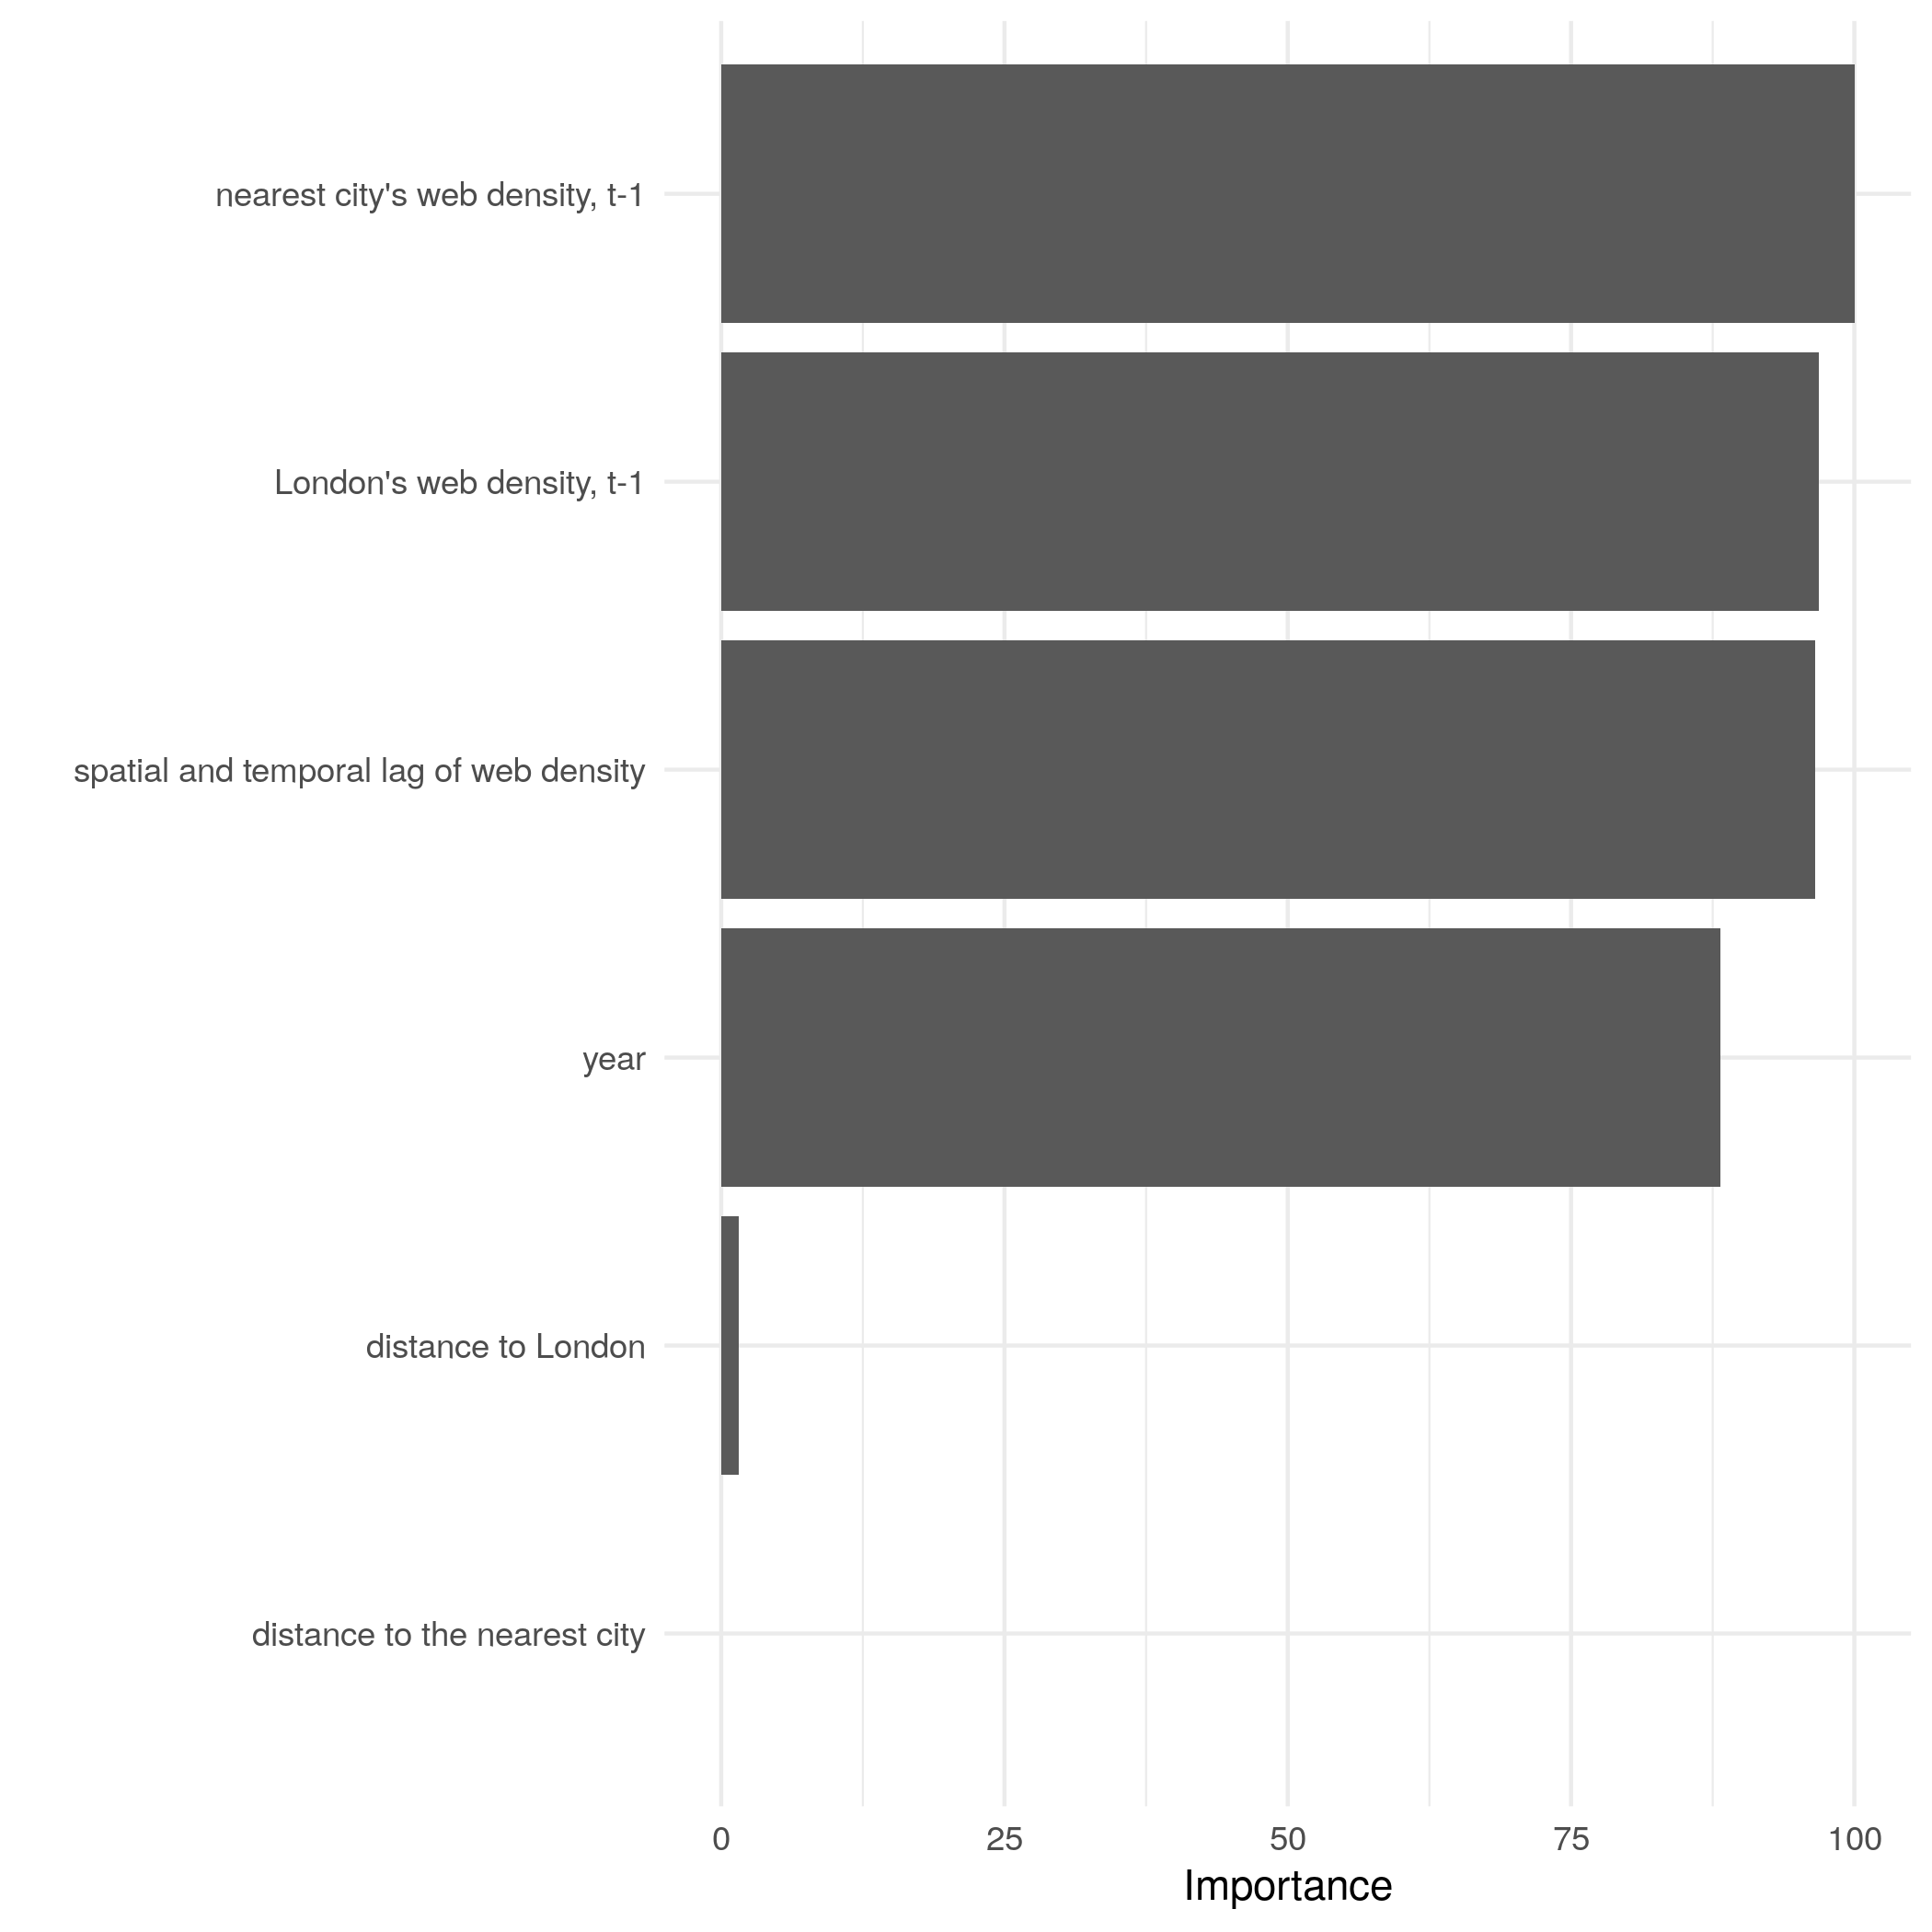
\includegraphics[width=1\textwidth,height=\textheight]{../../outputs/rf/figures/varimp_LA.png}

}

\caption{\label{var.imp.LAD}Variable importance, LAD}

\end{figure}%

\begin{figure}[H]

{\centering 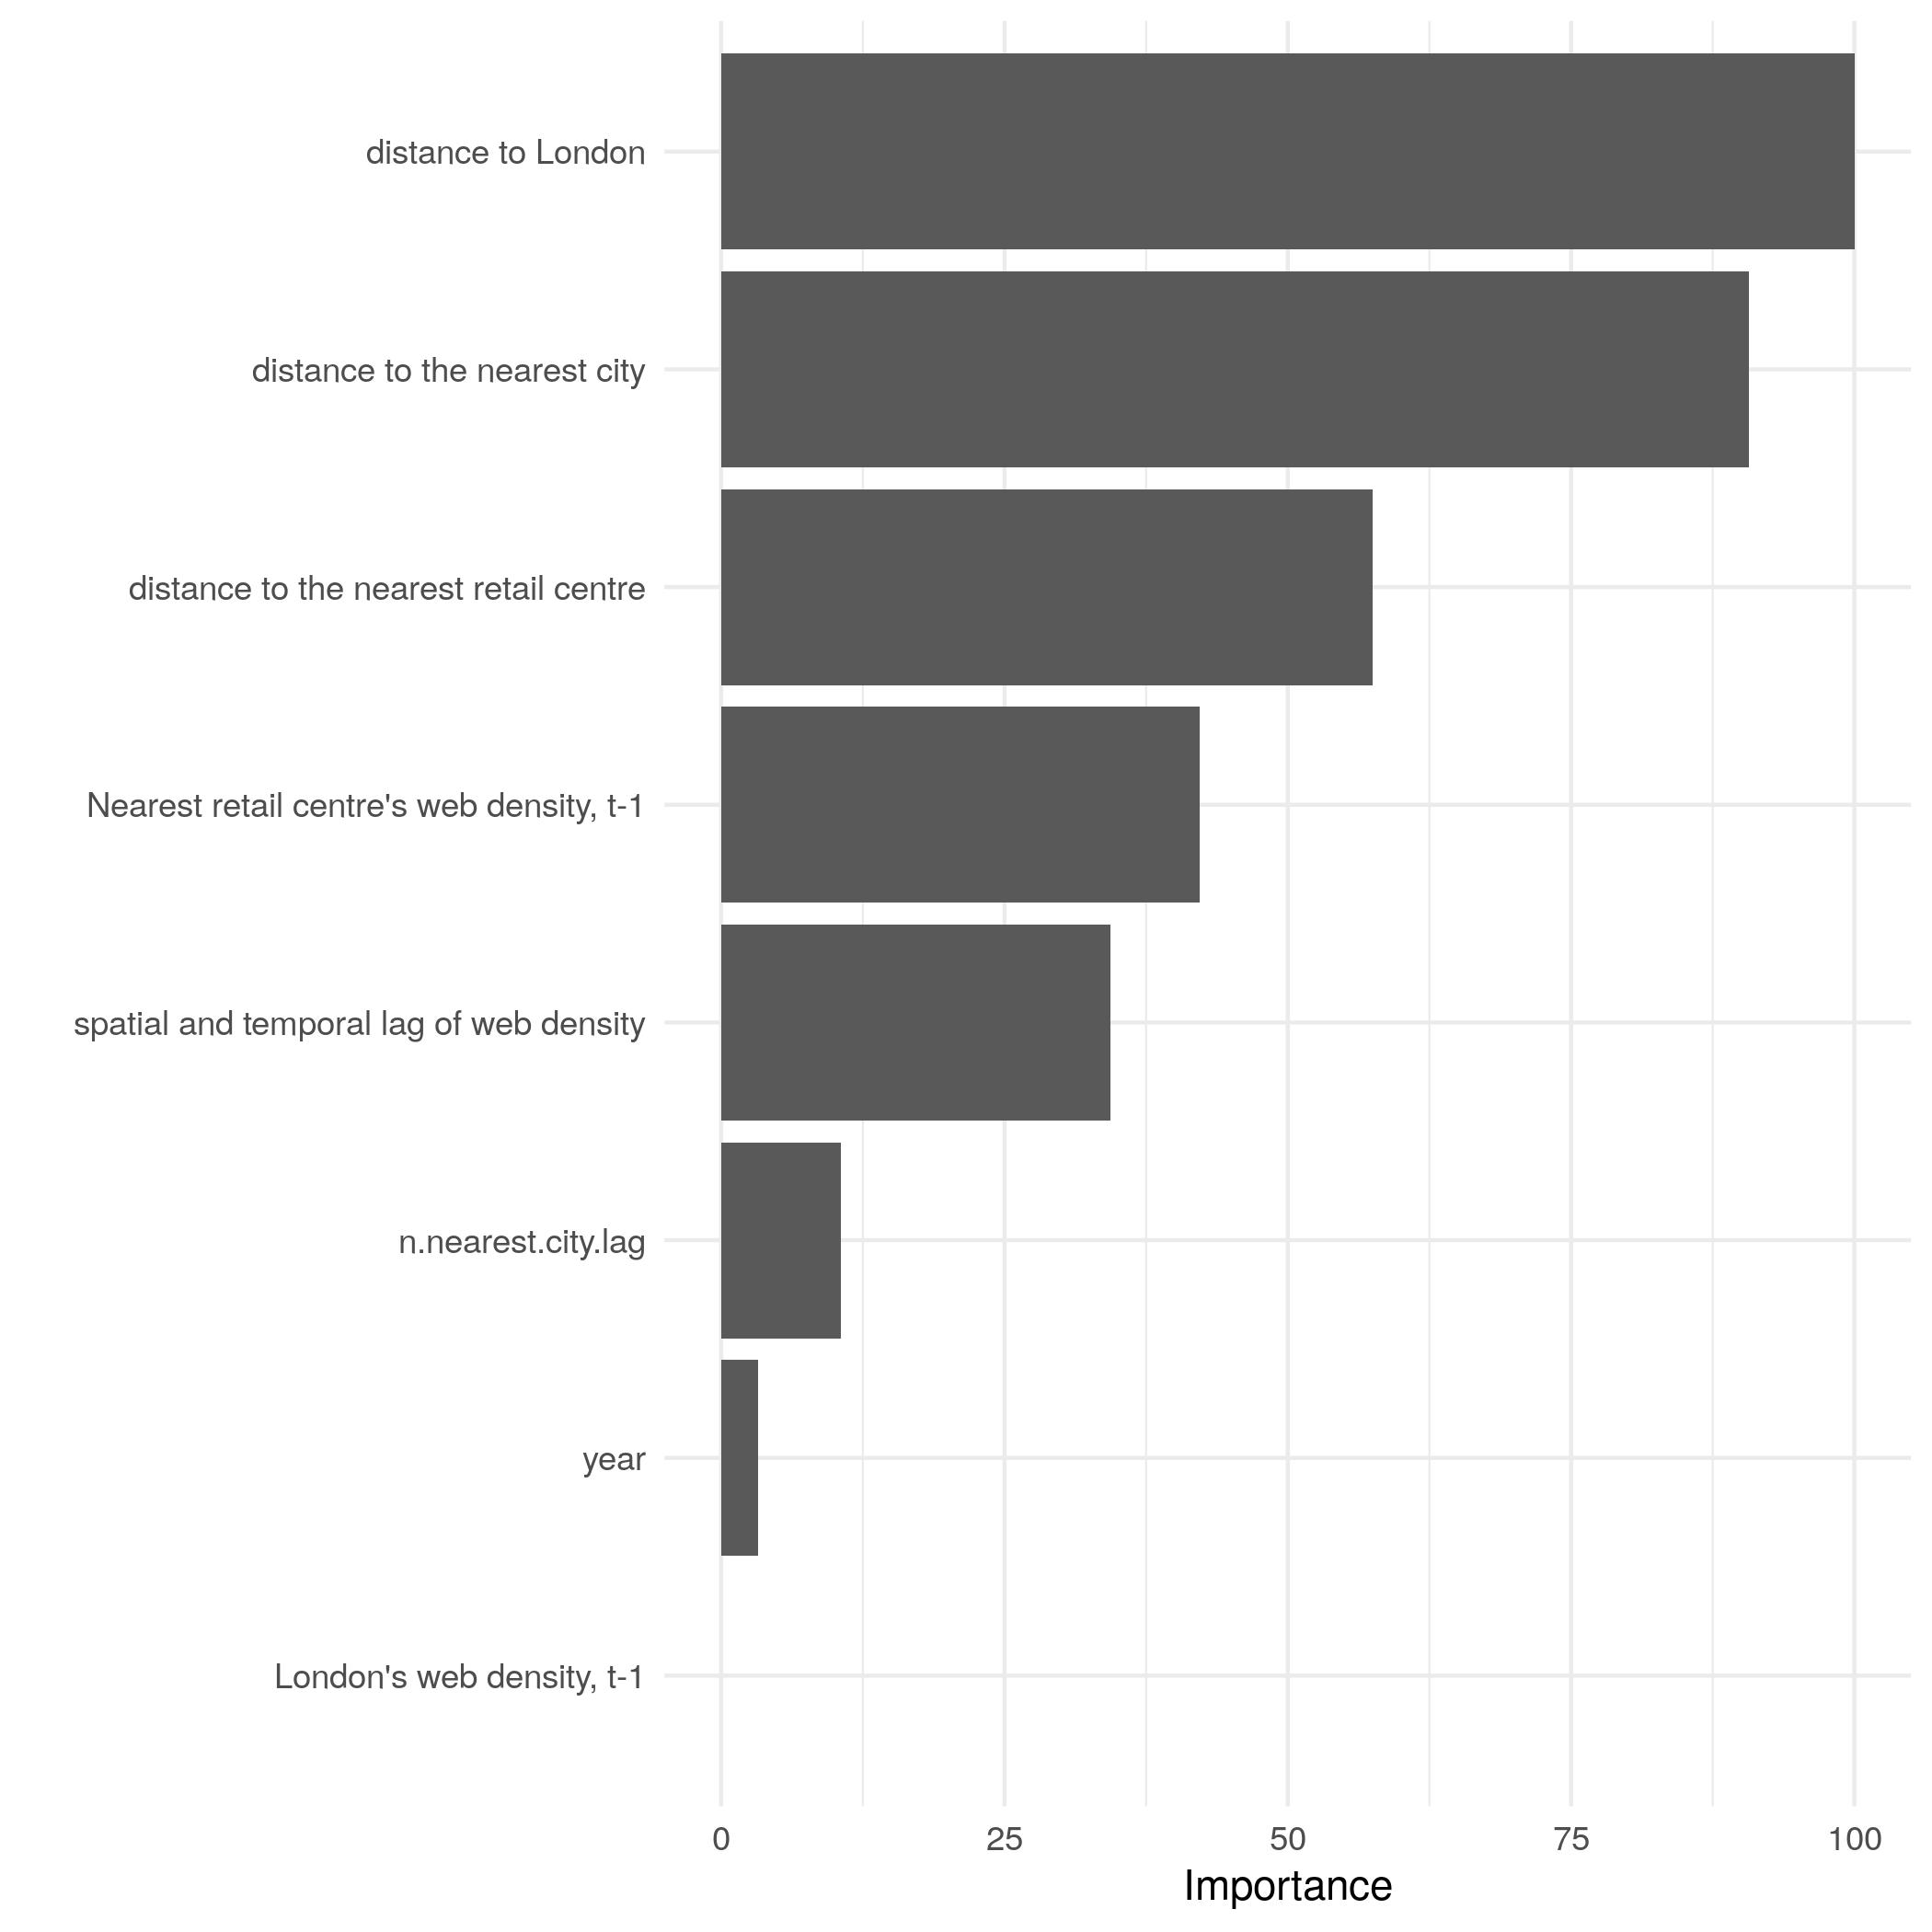
\includegraphics[width=1\textwidth,height=\textheight]{../../outputs/rf/figures/varimp_OA.png}

}

\caption{\label{var.imp.OA}Variable importance, OA}

\end{figure}%

Table \ref{table.regions} presents the results of the recursive hold out
models, which aim to highlight the potential regional heterogeneity of
the spatial processes behind the diffusion of web technologies. To begin
with, as highlighted before, there is a difference of magnitude of one
order between the LAD and the OA prediction errors, which is aligned
with previous results that employed all data points. What is of interest
here is the regional comparison. Table \ref{table.regions} illustrates
some striking similarities, but also a few significant differences. The
regions the web diffusion of which is better predicted using models
trained in the rest of the country are the same despite the scale of
analysis: South East, Wales, Yorkshire and The Humber and the North East
of England. In other words, these are the regions whose spatial
diffusion mechanisms of web technologies is closer to the country's
average. Despite the consistency across scales, this is a diverse set of
regions: \textbf{ADD CHARACTERISTICS}.

At the other end of the spectrum, Scotland's and the North West's web
diffusion mechanisms are consistently diverging from the country's
average. This should not come as a surprise as these regions are
characterised of high levels of rurality and remoteness. Similarly,
London diffusion mechanisms diverge from the country's average and this
is consistent across scales. London's uniqueness in UK's urban system
and economy is also reflected in the spatial diffusion mechanisms of web
technologies within its LAD and OA. It needs to be highlighted though
that the difference between the RSquared of LAD and OA is more that an
order of magnitude signaling how difficult is to predict diffusion at
such a small spatial scale. Northern Ireland is an interesting case.
While it ranks at the bottom of the scale when the models are trained
and tested on LAD data, when the modelling adopts the more granular OA
scale, the spatial mechanisms that shape the web diffusion within this
region appear to be closer to the country's average. At this scale,
proximity, or lack of, relative to the rest of the country become less
important and the internal to the region spatial structure predictors
start playing a more important role \textbf{CHECK NI OA model}.

\begin{longtable}[]{@{}
  >{\raggedright\arraybackslash}p{(\columnwidth - 8\tabcolsep) * \real{0.3731}}
  >{\raggedleft\arraybackslash}p{(\columnwidth - 8\tabcolsep) * \real{0.1940}}
  >{\raggedleft\arraybackslash}p{(\columnwidth - 8\tabcolsep) * \real{0.1343}}
  >{\raggedleft\arraybackslash}p{(\columnwidth - 8\tabcolsep) * \real{0.1791}}
  >{\raggedleft\arraybackslash}p{(\columnwidth - 8\tabcolsep) * \real{0.1194}}@{}}
\caption{Regional differences\label{table.regions}}\tabularnewline
\toprule\noalign{}
\begin{minipage}[b]{\linewidth}\raggedright
Region
\end{minipage} & \begin{minipage}[b]{\linewidth}\raggedleft
RSquared LAD
\end{minipage} & \begin{minipage}[b]{\linewidth}\raggedleft
Rank LAD
\end{minipage} & \begin{minipage}[b]{\linewidth}\raggedleft
RSquared OA
\end{minipage} & \begin{minipage}[b]{\linewidth}\raggedleft
Rank OA
\end{minipage} \\
\midrule\noalign{}
\endfirsthead
\toprule\noalign{}
\begin{minipage}[b]{\linewidth}\raggedright
Region
\end{minipage} & \begin{minipage}[b]{\linewidth}\raggedleft
RSquared LAD
\end{minipage} & \begin{minipage}[b]{\linewidth}\raggedleft
Rank LAD
\end{minipage} & \begin{minipage}[b]{\linewidth}\raggedleft
RSquared OA
\end{minipage} & \begin{minipage}[b]{\linewidth}\raggedleft
Rank OA
\end{minipage} \\
\midrule\noalign{}
\endhead
\bottomrule\noalign{}
\endlastfoot
South East & 0.947 & 1 & 0.134 & 2 \\
Wales & 0.916 & 2 & 0.131 & 3 \\
Yorkshire and The Humber & 0.906 & 3 & 0.144 & 1 \\
North East & 0.895 & 4 & 0.128 & 4 \\
West Midlands & 0.883 & 5 & 0.070 & 9 \\
East Midlands & 0.882 & 6 & 0.088 & 8 \\
East of England & 0.876 & 7 & 0.106 & 6 \\
South West & 0.864 & 8 & 0.117 & 5 \\
London & 0.805 & 9 & 0.055 & 10 \\
Scotland & 0.770 & 10 & 0.035 & 11 \\
North West & 0.664 & 11 & 0.017 & 12 \\
Nortern Ireland & 0.576 & 12 & 0.101 & 7 \\
\end{longtable}

\section{Discussion and conclusions}\label{discussion-and-conclusions}

contrary to results from future studies regarding social media
\citep{lengyel2020role}, web technologies did not exclusively spread
from a central location.


\renewcommand\refname{References}
  \bibliography{bibliography}


\end{document}
